\documentclass[]{scrartcl}

\usepackage{graphicx}
%%\usepackage{amsmath}

\usepackage{natbib}

%opening
\title{PHY 982 - HW 2}
\author{Xingze Mao \\ Zachary Matheson \\ Thomas Redpath}
\date{}

\begin{document}

\maketitle

\section*{Reactions and OMP parameters}

In this project, we study the cases of proton and neutron elastic scattering from $ ^{100} \mathrm{Mo} $ using the \texttt{FRESCO} code. Table~\ref{tab:entrance} lists the quantum numbers for the mass partition.

%\begin{equation}
%	^{100} \mathrm{Mo} (p,p) ^{100} \mathrm{Mo}
%	\label{eq:therxn}
%\end{equation}

%\begin{equation}
%	^{100} \mathrm{Mo} (n,n) ^{100} \mathrm{Mo}
%	\label{eq:therxn}
%\end{equation}


\begin{table}
\centering
	\begin{tabular}{ | c | c  c | }
\hline
	Projectile 1 & $p$ & $ J ^{\pi} = 1/2 ^+ $ \\
	Projectile 2 & $n$ & $ J ^{\pi} = 1/2 ^+ $ \\
\hline
	Target & $ ^{100} \mathrm{Mo} $ & $ J ^{\pi} = 0 ^+ $ \\
\hline
	\end{tabular}
	\caption{Entrance partition's quantum numbers.}
	\label{tab:entrance}
\end{table}

\subsection*{Proton elastic scattering: $E=5,50$ MeV}

\subsection*{Neutron elastic scattering: $E=5,50$ MeV}

\subsection*{Part II - Fitting}

To explore \texttt{fresco}'s application to fitting experimental data (via \texttt{sfresco}), we use the data for $ ^{100} \mathrm{Mo} (p,p)$ from \citep{Sinha1972}, which includes data for elastic scattering at three incident energies: $19.85,30.3,49.45$ MeV. We take the $49.45$ MeV data to include in our \texttt{sfresco} input file. These data are in units of mb/sr across 45 cm angles with a quoted error of $\sim 4 \%$. As the starting point for our fit, we take the real and imaginary volume parameters of \citep{Menet1971} for 49MeV incident energy (listed in Table~\ref{tab:init}). We then vary each of the six parameters one at a time to determine which gives the best fit (smallest $\chi ^2 / N$ and first derivative). We then fix this parameter by replacing the value in the potential defined in the \texttt{fresco} input file with this new value found by the fit. We proceed by individually varying the five remaining parameters to again determine which gives the smallest $\chi ^2 / N$ and first derivative, inputting this new value in the \texttt{fresco} input, repeating until all parameters have been fit. Table~\ref{tab:fitvol} reflects the order in which parameters were fit and the values, $\chi ^2 / N$ and first derivatives from each fit. The final fit compared to the data is shown in Figure~\ref{fig:fit1}.

Some observations:
\begin{itemize}
	\item First derivative depends mainly interval over which parameter is allowed to vary
	\item $\chi ^2 / N$ decreases slightly as each successive parameter is fixed
	\item Fits are not great: i will try adding the SO to the potential and/or different data
\end{itemize}

\begin{table}
\centering
	\begin{tabular}{ c | c c c | c c c  }
	$E _{\mathrm{in}}$ [MeV] & $ V _0$ & $ r _0$ & $ a _0$ & $W$ & $ r _{W} $ & $ a _{W} $\\
\hline
	49.0 &  47.0 &  1.16 &  0.75  &  5.6 & 1.37 &  0.51\\
\hline
	\end{tabular}
	\caption{Starting parameters for fitting real and imaginary volume.}
	\label{tab:initvol}
\end{table}


%% FIT VOLUME IMAGINARY %%
\begin{table}
\centering
	\begin{tabular}{ c | c | c c }
	Parameter & Value & $\chi ^2 / N$ & First Derivative\\
\hline
	$V$ & 43.8 & 155 & 0.3\\
	$W$ & 5.5 & 153 & 0.002\\
	$a _w$ & 0.42 & 151 & -2.91\\
	$a _0$ & 0.77 & 148 & 0.2\\
	$r _w$ & 1.36 & 144 & -0.52\\
	$r _0$ & 1.16 & 144 & 0.26\\
\hline
	\end{tabular}
	\caption{Results of fitting with a potential consisting of real and imaginary volume terms.}
	\label{tab:fitvol}
\end{table}

\begin{figure}
\centering
	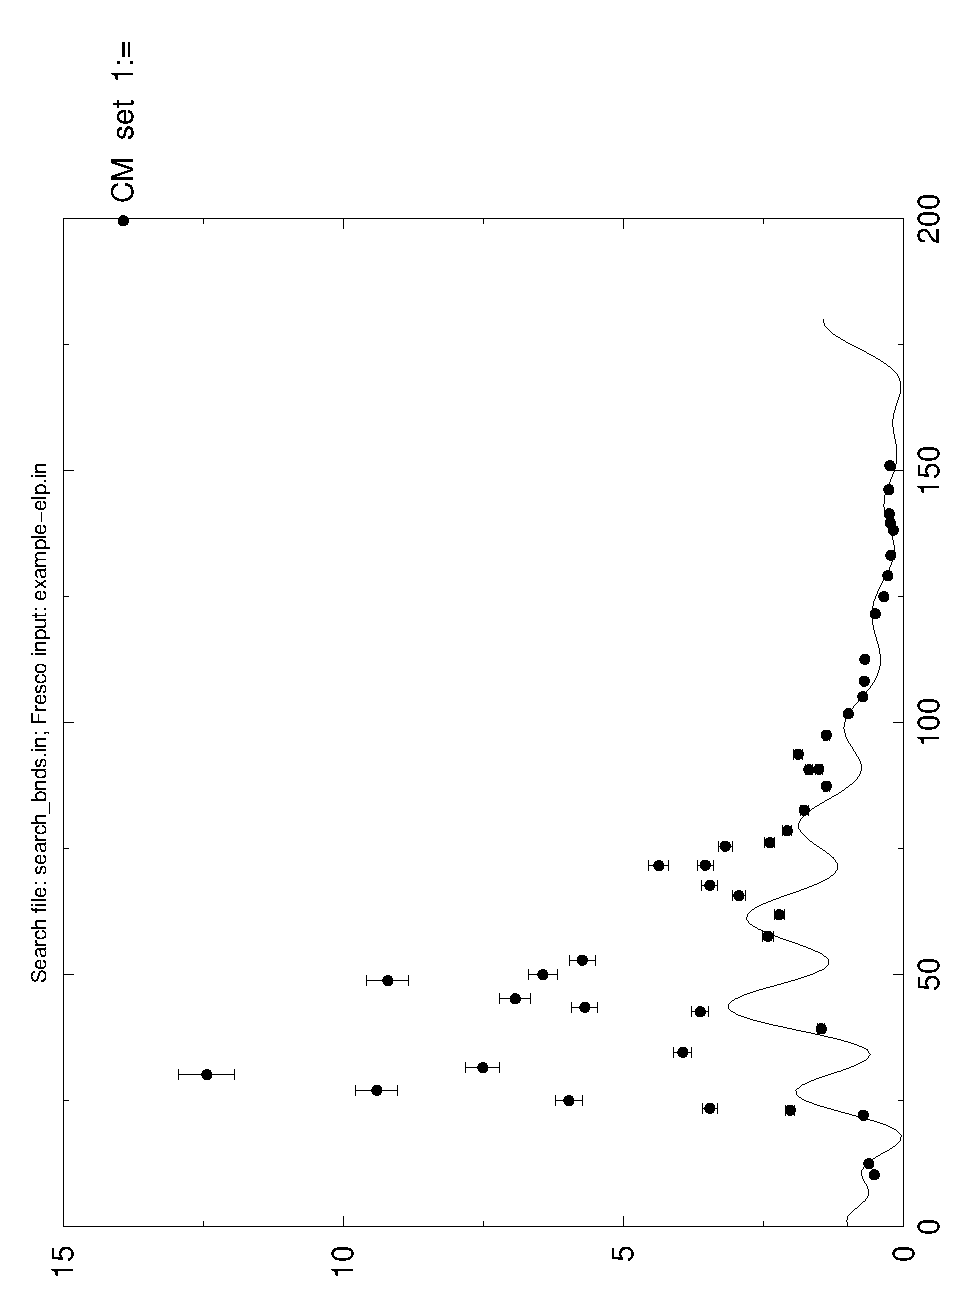
\includegraphics[width=0.78\textwidth,angle=270]{plots/searchV1.eps}
	\caption{The final fit of real and imaginary volume parameters to the proton elastic scattering data of \citep{Sinha1972}.}
	\label{fig:fit1}
\end{figure}

%% FIT SURFACE IMAGINARY %%
\begin{table}
\centering
	\begin{tabular}{ c | c c c | c c c  }
	$E _{\mathrm{in}}$ [MeV] & $ V _0$ & $ r _0$ & $ a _0$ & $W_s$ & $ r _{ws} $ & $ a _{ws} $\\
\hline
	49.0 &  47.0 &  1.16 &  0.75  &  4.2 & 1.37 &  0.51\\
\hline
	\end{tabular}
	\caption{Starting parameters for fitting with surface imaginary.}
	\label{tab:init}
\end{table}


\begin{table}
\centering
	\begin{tabular}{ c | c | c c }
	Parameter & Value & $\chi ^2 / N$ & First Derivative\\
\hline
	$a _{ws}$ & 1.49 & 258 & -2.9\\
	$r _{ws}$ & 1.18 & 226 & -0.001\\
	$a _0$ & 0.80 & 206 & -0.46\\
	$r _0$ & 1.21 & 192 & -0.44\\
	$W_s$ & 4.29 & 191 & -0.42\\
	$V$ & 47.1 & 190 & 0.19\\
\hline
	\end{tabular}
	\caption{Results fitting with a real volume and surface imaginary potential.}
	\label{tab:fitsurf}
\end{table}

\begin{figure}
\centering
	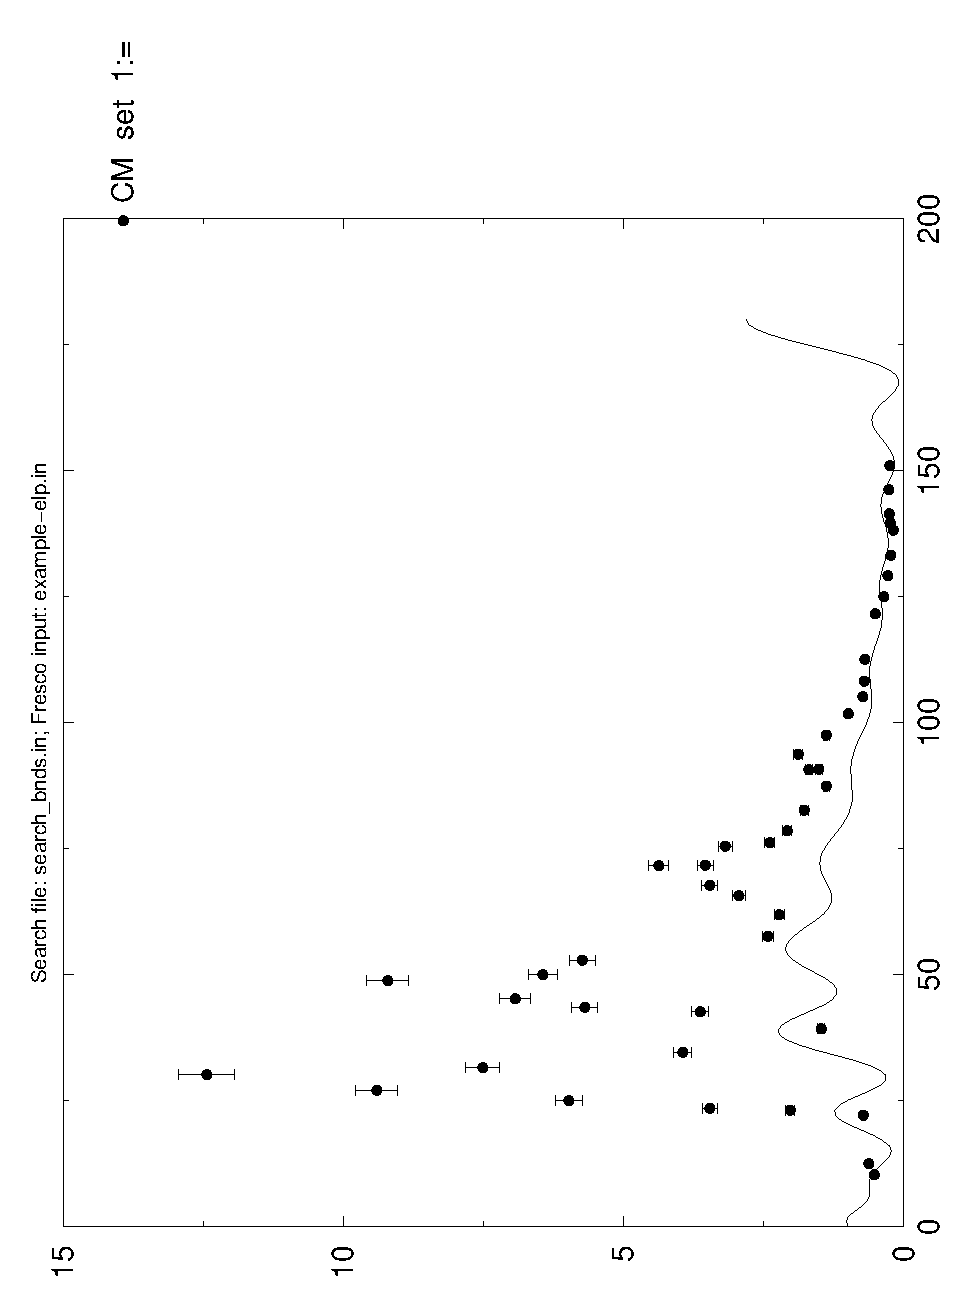
\includegraphics[width=0.78\textwidth,angle=270]{plots/searchS1.eps}
	\caption{The final fit of real volume and imaginary surface parameters to the proton elastic scattering data of \citep{Sinha1972}.}
	\label{fig:fit2}
\end{figure}



%\begin{figure}
%\centering
%	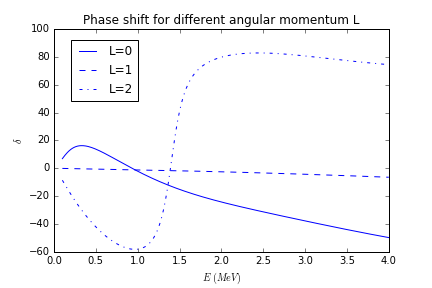
\includegraphics[width=0.85\textwidth]{figures/phase.png}
%	\caption{Phase shifts $\delta(E)$ for $l=0,1,2$. A weak resonance appears for $l=2$ near $E=1.4$ MeV with a width of $\sim 260$ keV.}
%	\label{fig:phase}
%\end{figure}

\clearpage


%%\bibliographystyle{apj}
\bibliographystyle{plain}
\bibliography{ref}

\end{document}
